\documentclass[aspectratio=169,11pt]{beamer}

\usepackage{graphicx}
\usepackage{booktabs}
\usepackage{array}
\usepackage{amsmath}
\usepackage{tikz}
\usetikzlibrary{shapes.geometric, arrows.meta, positioning}

% ---- clean light-grey minimalist theme ----
\usetheme{default}
\usefonttheme{serif}
\setbeamertemplate{navigation symbols}{}
\definecolor{bggray}{RGB}{237,237,237}
\definecolor{accent}{RGB}{40,72,120}
\setbeamercolor{background canvas}{bg=bggray}
\setbeamercolor{frametitle}{fg=black,bg=bggray}
\setbeamercolor{title}{fg=black}
\setbeamercolor{itemize item}{fg=accent}
\setbeamerfont{frametitle}{size=\LARGE,series=\mdseries}
\setbeamertemplate{frametitle}[default][center]
\setbeamertemplate{itemize item}{\textbullet}
\renewcommand{\arraystretch}{1.25}

\begin{document}

% ============ TITLE ============
\begin{frame}[plain]
\vspace{0.3cm}
\begin{center}
{\LARGE\bfseries RF-Based Drone Identification\\[2pt]
Using Machine Learning}\\[6pt]
{\footnotesize\color{gray}[23ET7PE3ML]}\\[6pt]
{\normalsize Department of Electronics and Telecommunication Engineering}\\[4pt]
{\footnotesize BMS College of Engineering, Bengaluru}
\end{center}
\vspace{0.6cm}
\begin{columns}[t]
\begin{column}{0.45\textwidth}
{\large Guided by}\\[3pt]
Dr. C Gururaj\\
Professor, ECE
\end{column}
\begin{column}{0.5\textwidth}
{\large Presented by}\\[3pt]
\begin{tabular}{@{}ll@{}}
Utkarsh Sinha & (1BM23ET055)\\
Vishal Joshy & (1BM23ET058)\\
Yash Gupta & (1BM23ET061)\\
\end{tabular}
\end{column}
\end{columns}
\end{frame}

% ============ INTRODUCTION + PROBLEM ============
\begin{frame}{Introduction and Problem Definition}
\begin{itemize}
\item Drones communicate with their controllers over radio-frequency (RF) links
in the 2.4~GHz band. Listening to these signals enables passive detection
without line of sight, unlike cameras or radar.
\item Detecting presence alone is insufficient; a practical system must also
identify the drone type and, where possible, its operating condition.
\item The 2.4~GHz band is shared with Wi-Fi and Bluetooth, so recorded signals
are noisy and classification is non-trivial.
\item Segments extracted from one recording are highly correlated; splitting
them across training and test sets inflates accuracy through data leakage.
\item \textbf{Objective:} classify drone presence, family, and operating
condition from the DroneRF dataset under a leakage-aware evaluation.
\end{itemize}
\end{frame}

% ============ METHODOLOGY (FLOWCHART) ============
\begin{frame}{Proposed Methodology}
\centering
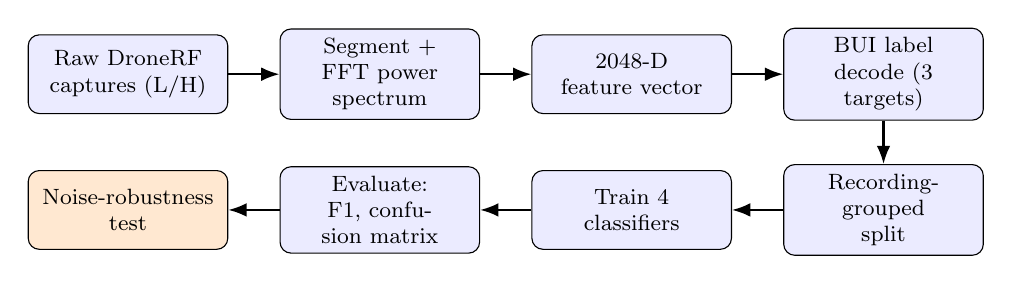
\begin{tikzpicture}[
  node distance=0.55cm and 0.65cm,
  box/.style={rectangle, draw, rounded corners, align=center,
    font=\footnotesize, minimum height=1.0cm, text width=2.3cm, fill=blue!8},
  save/.style={rectangle, draw, rounded corners, align=center,
    font=\footnotesize, minimum height=1.0cm, text width=2.3cm, fill=orange!18},
  arr/.style={-{Latex}, thick}
]
\node[box] (raw) {Raw DroneRF\\captures (L/H)};
\node[box, right=of raw] (seg) {Segment +\\FFT power spectrum};
\node[box, right=of seg] (feat) {2048-D\\feature vector};
\node[box, right=of feat] (label) {BUI label\\decode (3 targets)};
\node[box, below=of label] (split) {Recording-grouped\\split};
\node[box, left=of split] (train) {Train 4\\classifiers};
\node[box, left=of train] (eval) {Evaluate:\\F1, confusion matrix};
\node[save, left=of eval] (noise) {Noise-robustness\\test};
\draw[arr] (raw) -- (seg);
\draw[arr] (seg) -- (feat);
\draw[arr] (feat) -- (label);
\draw[arr] (label) -- (split);
\draw[arr] (split) -- (train);
\draw[arr] (train) -- (eval);
\draw[arr] (eval) -- (noise);
\end{tikzpicture}
\vspace{0.3cm}

\footnotesize Three classification targets are decoded from a single 5-digit
BUI filename code: presence (2 classes), family (4), and operating mode (10).
\end{frame}

% ============ DATASET + FEATURES ============
\begin{frame}{Dataset and Feature Extraction}
\begin{columns}[t]
\begin{column}{0.52\textwidth}
\textbf{DroneRF dataset}
\vspace{0.15cm}

\scriptsize
\begin{tabular}{|l|c|c|}
\hline
\textbf{Class} & \textbf{BUI} & \textbf{Modes} \\
\hline
Background & 00000 & 1 \\
\hline
Parrot Bebop & 10000--10011 & 4 \\
\hline
Parrot AR & 10100--10111 & 4 \\
\hline
DJI Phantom & 11000 & 1 \\
\hline
\end{tabular}
\vspace{0.2cm}

\footnotesize 227 recording pairs (low \texttt{L} + high \texttt{H} sub-bands),
2.4~GHz ISM band.
\end{column}
\begin{column}{0.46\textwidth}
\textbf{Feature extraction}
\begin{itemize}\footnotesize
\item Segment length $L = 100{,}000$ samples.
\item 2048-point FFT magnitude, upper 1024 bins:
\[\scriptstyle
X_f = \big|\mathrm{FFT}_M(x-\bar{x})\big|
\]
\item Low and high sub-bands joined and squared to a power spectrum.
\item \textbf{2048-D} vector per segment; \textbf{22{,}700} vectors total.
\end{itemize}
\end{column}
\end{columns}
\end{frame}

% ============ ALGORITHMS ============
\begin{frame}{Classification Models and Rationale}
\scriptsize
\begin{tabular}{|p{2.6cm}|p{4.3cm}|p{4.6cm}|}
\hline
\textbf{Model} & \textbf{Rationale for inclusion} & \textbf{Observed behaviour} \\
\hline
Logistic Regression & Linear baseline; a strong result implies a separable task &
Perfect on presence and family; weak on mode (0.375) \\
\hline
Random Forest & Bagging ensemble; captures non-linear structure &
Stable; marginally lower on family (0.898) \\
\hline
SVM (RBF kernel) & Models curved decision boundaries &
Strong on simple tasks; limited on mode (5k-sample cap) \\
\hline
XGBoost & Gradient-boosted trees; state-of-the-art on tabular data &
\textbf{Best overall}, and decisively best on the mode task \\
\hline
\end{tabular}
\vspace{0.25cm}

\footnotesize All four models perform near-identically on the easy tasks. They
separate only on the 10-class operating-mode task, where XGBoost leads, which is
where the comparison is meaningful.
\end{frame}

% ============ RESULTS + CONFUSION ============
\begin{frame}{Classification Results and Confusion Analysis}
\centering
\scriptsize
\begin{tabular}{|l|c|c|c|c|}
\hline
\textbf{Task} & \textbf{LR} & \textbf{RF} & \textbf{SVM} & \textbf{XGBoost} \\
\hline
Presence & 1.000 & 0.978 & 1.000 & 1.000 \\
\hline
Family & 0.999 & 0.898 & 0.977 & \textbf{1.000} \\
\hline
Mode (5-fold) & 0.375 & 0.378 & 0.160 & \textbf{0.492} \\
\hline
\end{tabular}

\vspace{0.2cm}
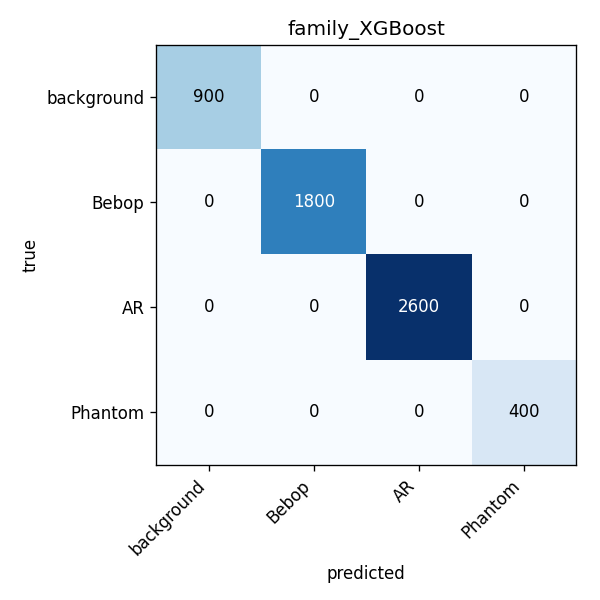
\includegraphics[height=0.44\textheight]{figs/cm_family.png}\hspace{0.5cm}
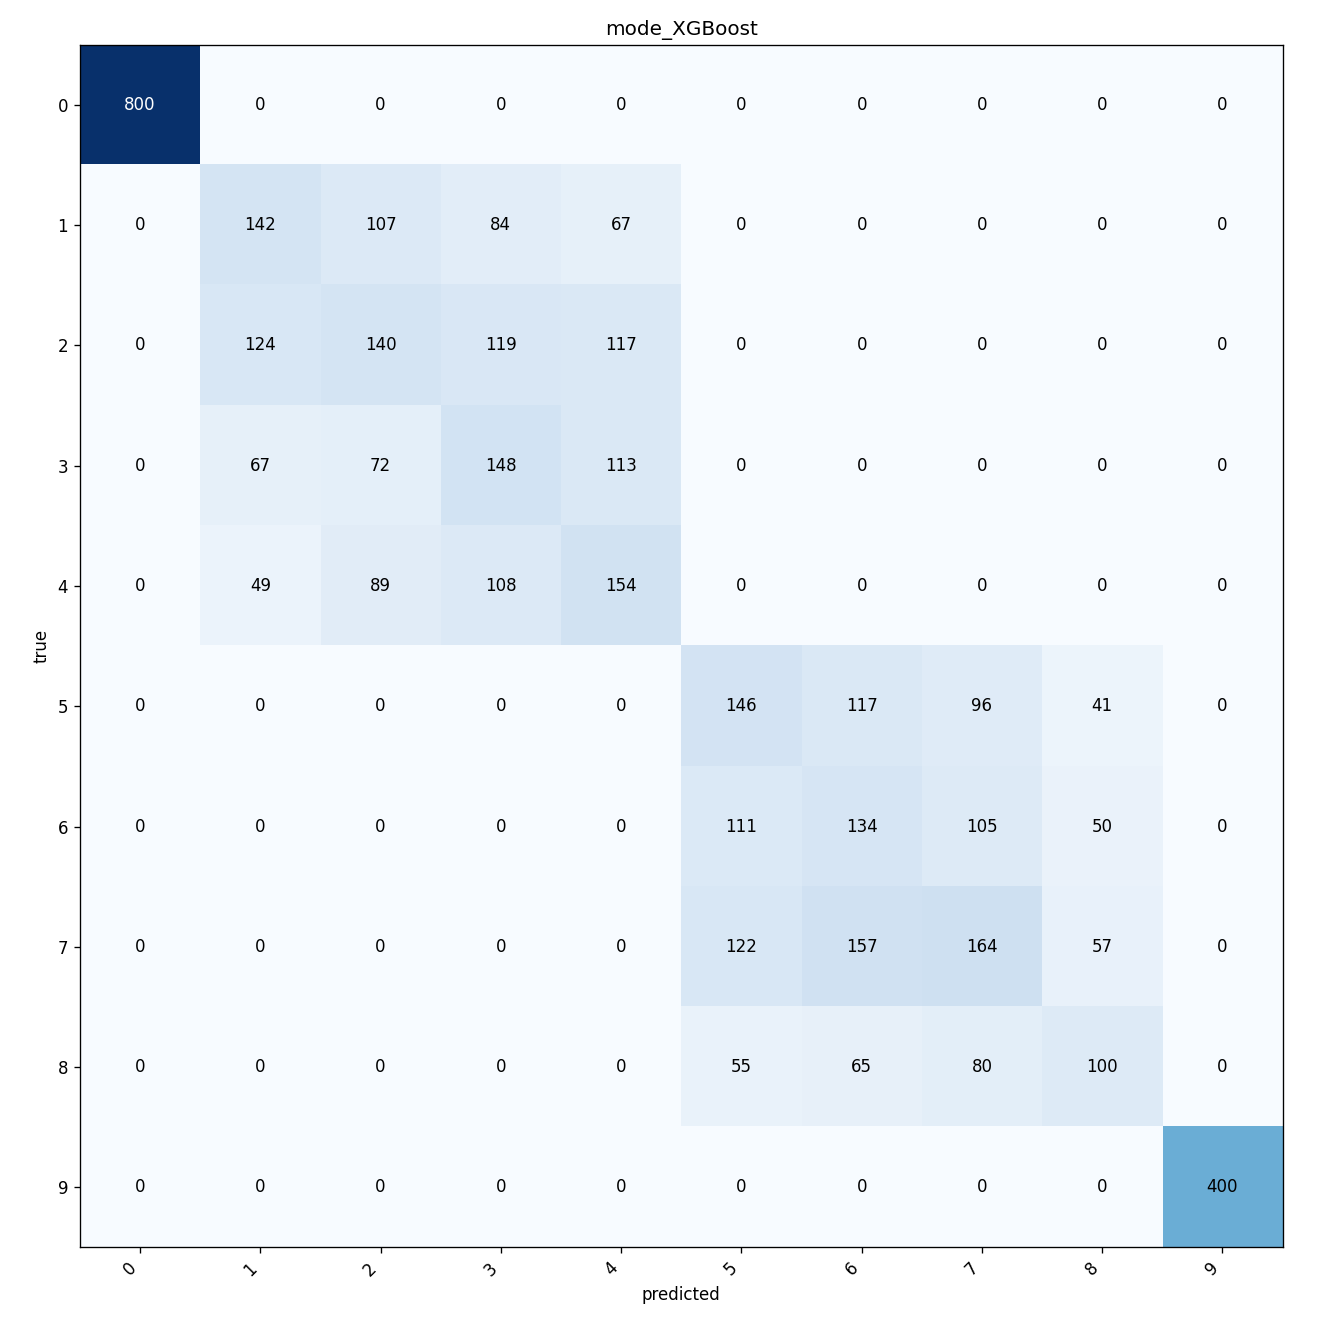
\includegraphics[height=0.44\textheight]{figs/cm_mode.png}

\footnotesize Macro-F1 by model (top). XGBoost confusion matrices: family is a
clean diagonal; the 10-class mode task shows residual confusion.
\end{frame}

% ============ NOISE ROBUSTNESS ============
\begin{frame}{Robustness Under Noise and Interference}
\begin{columns}[c]
\begin{column}{0.52\textwidth}
\centering
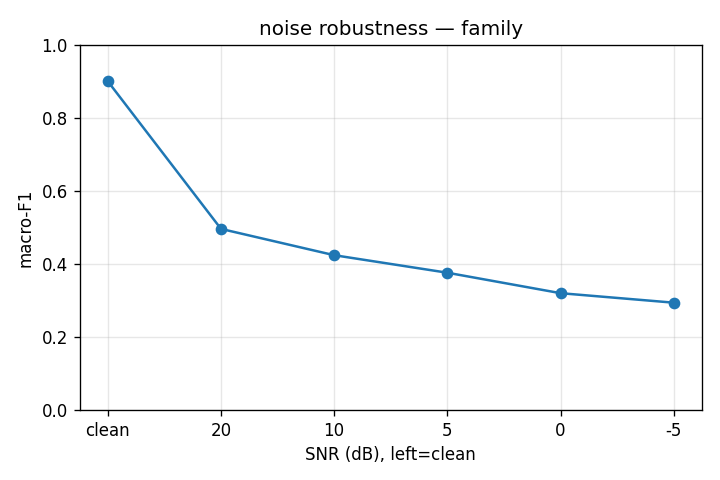
\includegraphics[width=\textwidth]{figs/noise.png}
\end{column}
\begin{column}{0.46\textwidth}
\scriptsize
\begin{tabular}{|l|c|}
\hline
\textbf{SNR} & \textbf{Macro-F1} \\
\hline
clean & 0.900 \\
20 dB & 0.496 \\
10 dB & 0.424 \\
5 dB & 0.376 \\
0 dB & 0.320 \\
$-5$ dB & 0.294 \\
\hline
\end{tabular}
\vspace{0.25cm}

\footnotesize Gaussian noise added to the family test set. Accuracy halves by
20~dB SNR, confirming that spectral features alone are not robust to the
interference present in the shared band.
\end{column}
\end{columns}
\end{frame}

% ============ ADVANTAGES + LIMITATIONS ============
\begin{frame}{Advantages and Limitations}
\begin{columns}[t]
\begin{column}{0.49\textwidth}
\textbf{Advantages}
\begin{itemize}\footnotesize
\item Passive detection without line of sight or lighting constraints.
\item Interpretable, low-cost models that train quickly.
\item Leakage-aware evaluation yields trustworthy metrics.
\item One pipeline answers all three classification questions.
\end{itemize}
\end{column}
\begin{column}{0.49\textwidth}
\textbf{Limitations}
\begin{itemize}\footnotesize
\item Operating-mode classification remains difficult (best F1 0.492).
\item Spectral features degrade sharply under heavy noise.
\item Only three drone families are represented in the dataset.
\item Dataset-based study; no live hardware or field deployment.
\end{itemize}
\end{column}
\end{columns}
\end{frame}

% ============ APPLICATIONS + CONCLUSION ============
\begin{frame}{Applications and Conclusion}
\begin{columns}[t]
\begin{column}{0.49\textwidth}
\textbf{Applications}
\begin{itemize}\footnotesize
\item Passive drone surveillance near airports and restricted zones.
\item Early warning for unauthorised drones at public events.
\item Low-cost monitoring on software-defined radios.
\item Drone-type identification for threat assessment.
\end{itemize}
\end{column}
\begin{column}{0.49\textwidth}
\textbf{Conclusion}
\begin{itemize}\footnotesize
\item Four classical models were compared across three tasks under a
leakage-aware split.
\item Presence and family are reliably classified; XGBoost leads the hard mode
task at 0.492.
\item A noise test quantified feature robustness under interference.
\item Classical models remain competitive with deep learning on this dataset.
\end{itemize}
\end{column}
\end{columns}
\end{frame}

% ============ LITERATURE SURVEY ============
\begin{frame}{Literature Survey}
\scriptsize
\begin{tabular}{|p{3.1cm}|p{2.7cm}|p{5.7cm}|}
\hline
\textbf{Paper} & \textbf{Method} & \textbf{Relevance to this work} \\
\hline
Al-Sa'd et al., 2019 (FGCS) & Deep neural networks &
Introduced the DroneRF dataset and the three-task structure adopted here. \\
\hline
Al-Emadi et al., 2020 & XGBoost, three tasks &
Closest prior work; confirms XGBoost's strength and the difficulty of the mode
task. \\
\hline
Ezuma et al., 2020 (OJ-COMS) & ML under Wi-Fi/BT interference &
Motivates the noise-robustness analysis in the shared 2.4~GHz band. \\
\hline
Medaiyese et al., 2022 (PMC) & Wavelet features + ML &
Principal alternative to the FFT/PSD features used in this project. \\
\hline
LUMEN, 2026 (Sensors) & PSD features, lightweight net &
Validates the power-spectral feature choice on constrained hardware. \\
\hline
Robustness study, 2024 (Sensors) & RF UAV detector robustness &
Establishes SNR-based degradation testing as standard evaluation practice. \\
\hline
\end{tabular}
\vspace{0.2cm}

\footnotesize\textbf{Research gap:} prior work is largely deep-learning-based or
omits an explicit leakage check. This project compares four interpretable
classical models across all three tasks under a recording-grouped split.
\end{frame}

% ============ REFERENCES ============
\begin{frame}{References}
\scriptsize
\begin{enumerate}
\item M. F. Al-Sa'd et al., ``RF-based drone detection and identification using
deep learning approaches,'' \textit{Future Generation Computer Systems},
vol. 100, 2019.
\item S. Al-Emadi, F. Al-Senaid, ``Drone detection using machine learning,''
\textit{Proc. IEEE IIT}, 2020.
\item M. Ezuma et al., ``Detection and classification of UAVs in the presence of
Wi-Fi and Bluetooth interference,'' \textit{IEEE OJ-COMS}, vol. 1, 2020.
\item O. O. Medaiyese et al., ``Wavelet transform analytics for RF-based UAV
detection,'' \textit{Pervasive and Mobile Computing}, vol. 82, 2022.
\item ``LUMEN: lightweight UAV network for PSD-based RF fingerprinting,''
\textit{Sensors}, vol. 26(10), 2026.
\item ``Robustness of deep-learning-based RF UAV detectors,'' \textit{Sensors},
vol. 24(22), 2024.
\item M. S. Allahham et al., ``DroneRF dataset,'' \textit{Data in Brief},
vol. 26, 2019.
\item M. Ezuma et al., ``Micro-UAV detection from RF fingerprints,''
\textit{Proc. IEEE Aerospace Conf.}, 2019.
\end{enumerate}
\end{frame}

\end{document}
